\setlength{\columnsep}{3pt}
\begin{flushleft}
\bigskip

\begin{itemize}
	\item The \textbf{/etc/hosts} file is used to \textbf{temporarily} resolve host names to IP addresses or the reverse. 
	\item \textbf{/etc/hosts} \textbf{do not} perform permanent name resolution like DNS server.
	\begin{figure}[h!]
		\centering
		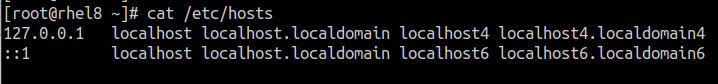
\includegraphics[scale=.45]{content/chapter14/images/hosts.png}
		\caption{Content of /etc/hosts file}
		\label{fig:hosts}
	\end{figure}		

	\item You can resolve your hostname to IP address by adding an entry to this file as shown:
	\begin{figure}[h!]
		\centering
		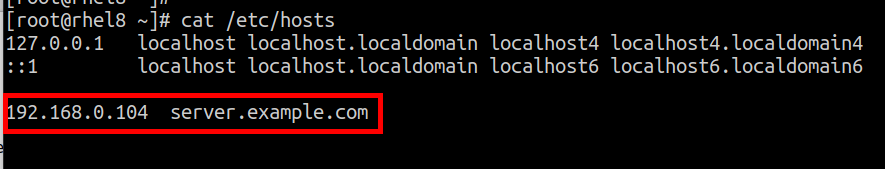
\includegraphics[scale=.35]{content/chapter14/images/hosts3.png}
		\caption{Add entry to /etc/hosts file}
		\label{fig:hosts3}
	\end{figure}		
	
	\item Test host name resolution with the /etc/hosts file using below command:
	\bigskip
		\begin{tcolorbox}[breakable,notitle,boxrule=-0pt,colback=pink,colframe=pink]
		\color{black}
		\fontdimen2\font=1em
		Syntax: getent hosts hostname
		\fontdimen2\font=4pt
	\end{tcolorbox}
	If an entry is not found in that file, the \textbf{getent} looks for the information from a DNS
	nameserver.
	\newline
	Eg:
	\bigskip
	\begin{tcolorbox}[breakable,notitle,boxrule=-0pt,colback=black,colframe=black]
		\color{green}
		\fontdimen2\font=1em
		\# getent hosts server.example.com
		\newline
		\color{white}
		fe80::a00:27ff:fe95:49b4 server.example.com
		\fontdimen2\font=4pt
	\end{tcolorbox}
	\newpage
	\item Test host name resolution that are resolved only using DNS and not \textbf{/etc/hosts}:
	\bigskip
	\begin{tcolorbox}[breakable,notitle,boxrule=-0pt,colback=pink,colframe=pink]
		\color{black}
		\fontdimen2\font=1em
		Syntax: host hostname
		\fontdimen2\font=4pt
	\end{tcolorbox}
	Eg:
	\bigskip
	\begin{figure}[h!]
		\centering
		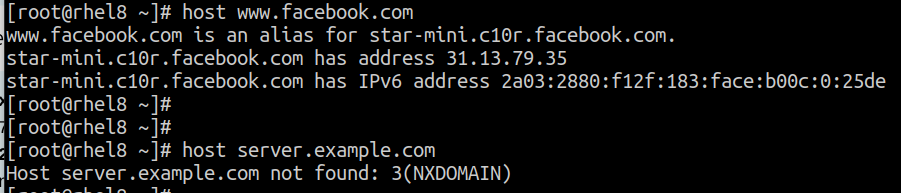
\includegraphics[scale=.35]{content/chapter14/images/hosts2.png}
		\caption{Sample output}
		\label{fig:hosts2}
	\end{figure}		

	
\end{itemize}



\end{flushleft}
\newpage


